\chapter{Seconda istanziazione}
\section{Schema a blocchi e definizione dei segnali IN/OUT}
A partire da quanto esposto nel precedente capitolo segue lo schema di seconda istanziazione della CPU.
\newpage
\begin{figure}[H]
	\centering
	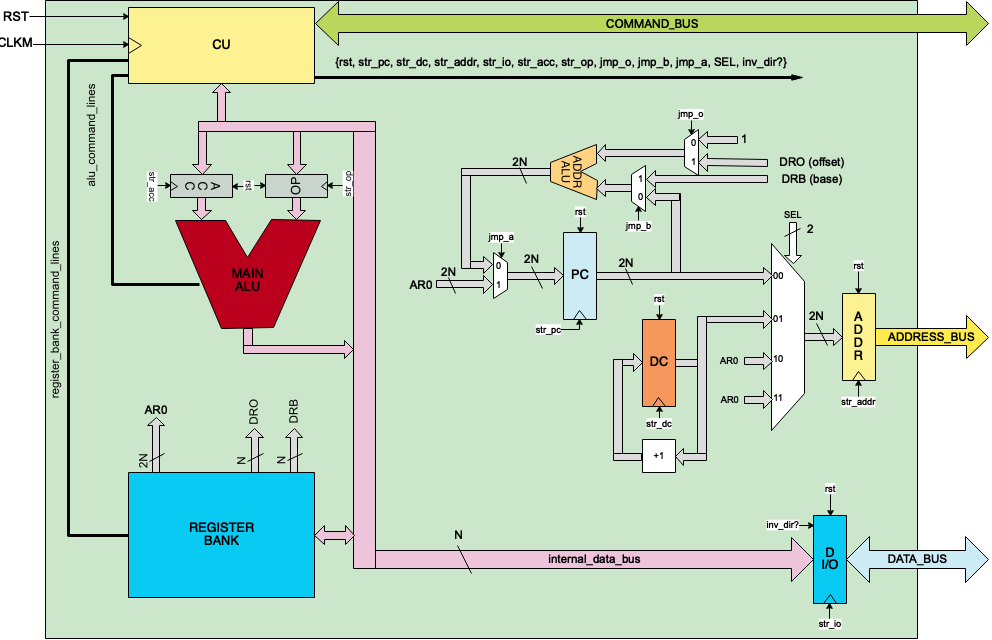
\includegraphics[scale=0.60, angle=90]{2_seconda_istanziazione}
	\label{fig:seconda_istanziazione}
\end{figure}

\newpage
\section{Definizione ulteriore dei segnali interni}
\begin{itemize}
	\item \textit{rst}: \{0: funzionamento normale; 1: reset prioritario per i registri interni\}.
	\item \textit{str\_pc}: strobe per il registro PC.
	\item \textit{str\_dc}: strobe per il registro DC.
	\item \textit{str\_addr}: strobe per il registro address.
	\item \textit{str\_io}: strobe per il registro di I/O.
	\item \textit{str\_acc}: strobe per il registro accumulatore.
	\item \textit{str\_op}: strobe per il registro operando.
	\item \textit{jmp\_o}: segnale di comando per il mux. \{0: uscita = 1, 1: uscita = \textit{DRO}\}.
	\item \textit{jmp\_b}: segnale di comando per il mux. \{0: uscita = PC, 1: uscita = \textit{DRB}\}.
	\item \textit{jmp\_a}: segnale di comando per il mux. \{0: uscita = \textit{ALU\_ADDR\_OUT}, 1: uscita = \textit{AR0}\}.
	\item \textit{\textbf{SEL}}: 2 bit. Segnale di comando per il mux selezione indirizzo. Vedi \ref{2_tabella_SEL}.
	\item \textit{inv\_dir?}: \{0: registro I/O in funzionamento IN $\rightarrow$ OUT; 1: registro I/O in funzionamento OUT $\rightarrow$ IN\}.
	\item \textit{\textbf{alu\_command\_lines}}: linee di controllo per la ALU principale.
	\item \textit{\textbf{register\_bank\_command\_lines}}: linee di controllo per il register bank.
	\item \textit{\textbf{internal\_data\_lines}}: Bus dati interno a N bit.
\end{itemize}

\section{Ulteriori considerazioni di seconda istanziazione}
Per ciò che concerne l'indirizzamento della memoria si può notare che il registro indirizzo è pilotato da un mux 4-1, controllato tramite \textit{\textbf{SEL}}. \textit{\textbf{SEL}} è un segnale a 2 bit proveniente dalla CU ed il controllo del mux è schematizzato nella seguente tabella:
\begin{table}[H]
	\centering
	\footnotesize
	\fontsize{10}{18}\selectfont
	\begin{tabular}{|p{1.5cm}|p{1.5cm}|p{2.5cm}|}
		\hline
		\multicolumn{1}{|c|}{\textit{$SEL_1$}} &
		\multicolumn{1}{c|}{\textit{$SEL_0$}} & 
		\multicolumn{1}{c|}{SORGENTE ADDR}\\
		
		\hline
		\multicolumn{1}{|c|}{0} &
		\multicolumn{1}{c|}{0} & 
		\multicolumn{1}{c|}{\textbf{PC}}\\
		
		\hline
		\multicolumn{1}{|c|}{0} &
		\multicolumn{1}{c|}{1} & 
		\multicolumn{1}{c|}{\textbf{DC}}\\
		
		\hline
		\multicolumn{1}{|c|}{1} &
		\multicolumn{1}{c|}{0} & 
		\multicolumn{1}{c|}{\textbf{AR0}}\\
		
		\hline
		\multicolumn{1}{|c|}{1} &
		\multicolumn{1}{c|}{1} & 
		\multicolumn{1}{c|}{\textbf{AR0}}\\ \hline
	\end{tabular}
	\caption{Indirizzamento della memoria}
	\label{2_tabella_SEL}
\end{table}
\noindent
Questo perché, come detto, è necessario avere tre possibili sorgenti per l'indirizzamento della memoria. Il valore di indirizzamento proviene da PC, DC oppure da AR0, nei casi in cui $SEL_1$ = 1. AR0 è uno dei tre registri presenti nel banco d'appoggio con \textquotedblleft funzione speciale", ossia connesso ad un bus esterno accessibile in modo prioritario, proprio per avere la possibilità di realizzare funzioni come l'indirizzamento della memoria o il caricamento del valore del salto nel caso della jump.

\section{Dimensionamento interno dei blocchi di seconda istanziazione}
\subsection{Register bank}
\begin{figure}[H]
	\centering
	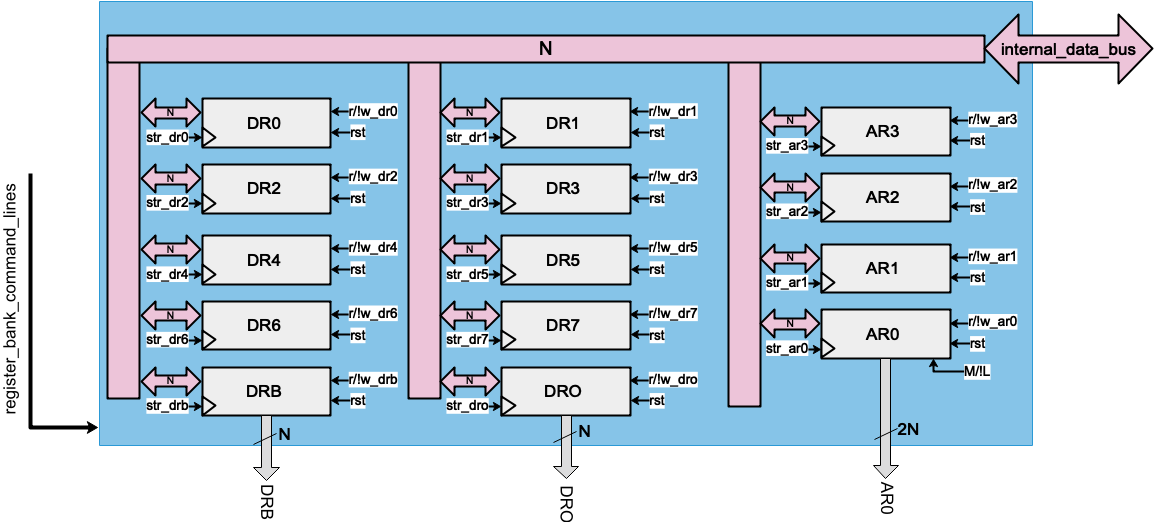
\includegraphics[scale=0.35, angle=0]{2_register_bank}
	\label{fig:register_bank}
\end{figure}
Il register bank contiene 14 registri di supporto al calcolo, di cui 4 riservati al calcolo degli indirizzi. Tra di essi vi sono tre registri accessibili esternamente attraverso altrettanti bus dedicati. Tali registri sono:
\begin{itemize}
	\item DRB: nel caso dell'operazione JBO in questo registro è presente il valore relativo alla base da sommare all'offset per il calcolo dell'indirizzo di salto.
	\item DRO: nel caso delle operazioni di JPO o JBO in questo registro è presente il valore relativo all'offset da sommare al PC o alla base per il calcolo dell'indirizzo di salto.
	\item AR0: in questo registo è presente il valore da dare al PC nel caso di jump immediata, oppure il valore da fornire alla memoria nel caso di RD o WR. Questo registro ha dimensione 2N bit per garantire l'indirizzamento a tutta la memoria, tuttavia è collegato attraverso il bus dati interno solo agli ultimi N bit. Attraverso il comando denominato $M/\overline{L}$ indirizzare il bus dati in scrittura ai primi N flip-flop o agli ultimi N flip-flop che compongono tale registro, per garantire il caricamento su tutto lo spazio dei 2N bit tramite bus a N bit. Di seguito sarà presentato lo schema interno-
\end{itemize}
Ogni registro componente il register bank è pilotato singolarmente attraverso una terna di segnali: \{\textit{str\_xxx}, \textit{rst}, \textit{r/$\overline{w}$\_xxx}\}. Nel caso del registro AR0 è presente anche il segnale $M/\overline{L}$ il cui impiego è necessario per avere la possibilità di scrivere o leggere separatemente i LSH (Least Significant Heap) o gli MSH (Most Significant Heap), ossia gli ultimi/primi N bit del registro. Dettagli del funzionamento del registro AR0 saranno esposti in seguito.\\
L'insieme dei segnali di controllo è stato schematizzato nella figura con l'insieme di linee denominato \textit{\textbf{register\_bank\_command\_lines}}.\\
Ogni registro che compone il register bank è inoltre di tipo bidirezionale a singolo bus, per avere la possibilità di essere letto o scritto attraverso il bus dati interno. Lo schema interno del generico registro, supposto N=4 bit, è rappresentato nella figura seguente.
\begin{figure}[H]
	\centering
	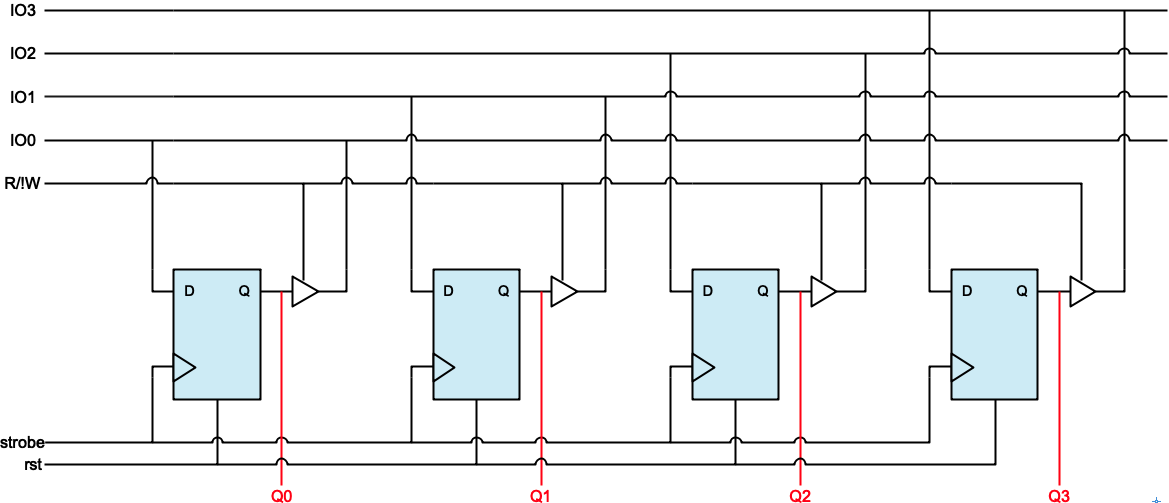
\includegraphics[scale=0.32, angle=0]{2_registro_bidir}
	\label{fig:registro_bidir}
\end{figure}
\noindent
In questo schema il comando $R/ \overline{W}$ definisce se il registro è abilitato alla lettura (1) o alla scrittura (0), in modo che il bus possa essere bidirezionale. Quando un registro non è utilizzato deve essere mantenuto in modalità scrittura ($R/ \overline{W} = 0$) per far si che i tri-state d'uscita siano disabilitati in modo da non interferire col controllo del bus da parte di altre entità ad esso collegate.
\\
In rosso invece sono rappresentate le linee d'uscita disponibili solamente per i registri con accesso speciale DRO e DRB, che costituiscono i bus dedicati discussi in precedenza.\\
Lo schema interno del registro AR0 (rappresentato per N=2 bit) è invece il seguente. Si ricorda che la dimensione di tale registro è pari a 2N bit, dunque:
\begin{figure}[H]
	\centering
	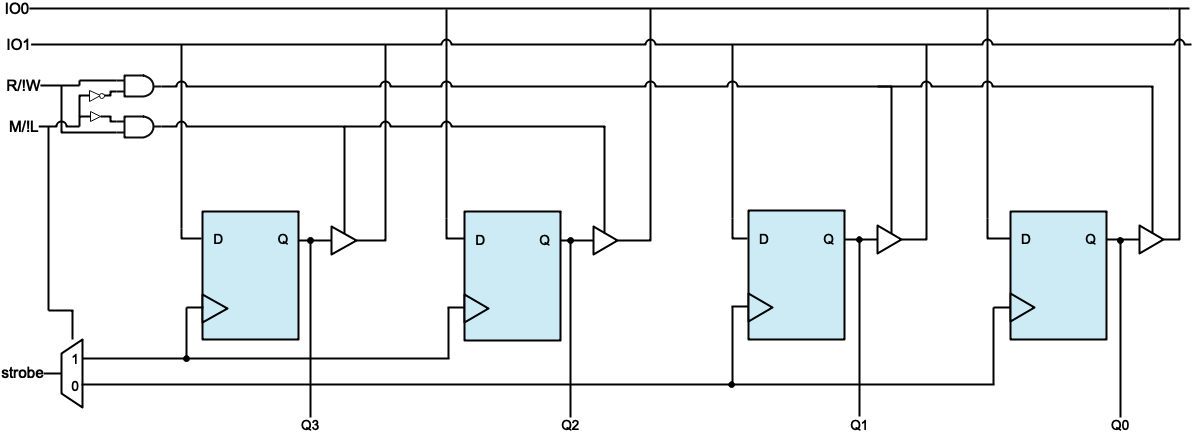
\includegraphics[scale=0.32, angle=0]{2_AR0}
	\label{fig:AR0}
\end{figure}
\noindent
Si può notare il demultiplexer interno che permette lo smistamento del segnale di strobe indipendentemente al primo o al secondo gruppo di flip-flop e la rete logica che pilota i tri-state che realizza la seguente funzione.
\begin{table}[H]
	\centering
	\fontsize{10}{18}\selectfont
	\begin{tabular}{|p{5mm}|p{5mm}|p{25mm}|}
		\hline
		\multicolumn{1}{|c|}{\textit{$R/\overline{W}$}} &
		\multicolumn{1}{c|}{\textit{$M/\overline{L}$}} & 
		\multicolumn{1}{c|}{\textbf{modalità}}\\
		
		\hline
		\multicolumn{1}{|c|}{0} &
		\multicolumn{1}{|c|}{0} & 
		\multicolumn{1}{c|}{lettura LSH}\\
		
		\hline
		\multicolumn{1}{|c|}{0} &
		\multicolumn{1}{|c|}{1} & 
		\multicolumn{1}{c|}{lettura MSH}\\
		
		\hline
		\multicolumn{1}{|c|}{1} &
		\multicolumn{1}{|c|}{0} & 
		\multicolumn{1}{c|}{scrittura LSH}\\
		
		\hline
		\multicolumn{1}{|c|}{1} &
		\multicolumn{1}{|c|}{1} & 
		\multicolumn{1}{c|}{scrittura MSH}\\ \hline
	\end{tabular}
	\caption{Modalità di funzionamento registro AR0}
\end{table}
\noindent
Omesso dal disegno, ma presente, il clear prioritario dei flip-flop connesso al segnale esterno di \textit{reset}.
\subsection{Unità di controllo: CU}